\let\negmedspace\undefined
\let\negthickspace\undefined
\documentclass[journal]{IEEEtran}
\usepackage[a5paper, margin=10mm, onecolumn]{geometry}
%\usepackage{lmodern} % Ensure lmodern is loaded for pdflatex
\usepackage{tfrupee} % Include tfrupee package

\setlength{\headheight}{1cm} % Set the height of the header box
\setlength{\headsep}{0mm}     % Set the distance between the header box and the top of the text

\usepackage{gvv-book}
\usepackage{gvv}
\usepackage{cite}
\usepackage{amsmath,amssymb,amsfonts,amsthm}
\usepackage{algorithmic}
\usepackage{graphicx}
\usepackage{textcomp}
\usepackage{xcolor}
\usepackage{txfonts}
\usepackage{listings}
\usepackage{enumitem}
\usepackage{mathtools}
\usepackage{gensymb}
\usepackage{comment}
\usepackage[breaklinks=true]{hyperref}
\usepackage{tkz-euclide} 
\usepackage{listings}
% \usepackage{gvv}                                        
\def\inputGnumericTable{}                                 
\usepackage[latin1]{inputenc}                                
\usepackage{color}                                            
\usepackage{array}                                            
\usepackage{longtable}                                       
\usepackage{calc}                                             
\usepackage{multirow}                                         
\usepackage{hhline}                                           
\usepackage{ifthen}                                           
\usepackage{lscape}
\begin{document}

\bibliographystyle{IEEEtran}
\vspace{3cm}




\title{
%	\logo{
GATE - 2018- XE

\large{EE1030 : Matrix Theory}

Indian Institute of Technology Hyderabad
%	}
}
\author{Satyanarayana Gajjarapu

AI24BTECH11009
}	





\maketitle




\bigskip

\renewcommand{\thefigure}{\theenumi}
\renewcommand{\thetable}{\theenumi}


\section{27 - 39}


\begin{enumerate}
\item If the stream function $\brak{\psi\brak{x,y}}$ for a two-dimensional incompressible flow field is given as $2y\brak{x^2 - y^2}$, the corresponding velocity field is 
\begin{enumerate}
    \item $\overrightarrow{V} = 2\brak{x^2 - 3y^2}\hat{i} + 4xy\hat{j}$
    \item $\overrightarrow{V} = 2\brak{x^2 - 3y^2}\hat{i} - 4xy\hat{j}$
    \item $\overrightarrow{V} = 2\brak{x^2y}\hat{i} - 4xy\hat{j}$
    \item $\overrightarrow{V} = 2\brak{x^2y}\hat{i} + 4xy\hat{j}$ \\
\end{enumerate}
\item Water is flowing in two different tubes of diameters $D$ and $2D$, with the same velocity. The ratio of laminar friction factors for the larger diameter tube to the smaller diameter tube is 
\begin{enumerate}
    \item 0.5
    \item 1.0
    \item 2.0
    \item 4.0 \\
\end{enumerate}
\item If the velocity field is $\overrightarrow{V} = x^2y\hat{i} + 4xy\hat{j}$ m/s, vorticity of the fluid element in the field at \brak{x=1, y=2} in $\text{s}^{-1}$ is $\_\_\_\_$. \\
\item A pitot-static tube is used to measure air velocity in a duct by neglecting losses. The density of air is 1.2 kg/$\text{m}^3$. If the difference between the total and static pressures is 1 kPa, the velocity of air at the measuring location, in m/s, is $\_\_\_\_$. \\
\item A parallelepiped of (2 m $\times$ 2 m) square cross-section and 10 m in length, is partially floating in water upto a depth of 1.2 m, with its longest side being horizontal. The specific gravity of the block is
 \begin{enumerate}
    \item 0.8
    \item 0.6
    \item 0.5
    \item 0.4 \\
\end{enumerate}
\item The velocity field in a two-dimensional, unsteady flow is given by $\overrightarrow{V}\brak{x,y,t} = 2xy^2\hat{i} + 3xyt\hat{j}$ m/s. The magnitude of acceleration of a fluid particle located at $x = 1$ m, $y = 1$ m at the time $t = 1$ s, in m/$\text{s}^2$, is
\begin{enumerate}
    \item 16.0
    \item 18.1
     \item 24.1
    \item 34.1 \\
\end{enumerate}
\item In a two-dimensional, incompressible and irrotational flow, fluid velocity \brak{v} in the $y$-direction is given by $v = 2x - 5y$. The velocity \brak{u} in the $x$-direction is 
\begin{enumerate}
   \item $u = 2x - 5y$
   \item $u = 2x + 5y$
   \item $u = 5x + 2y$
   \item $u = 5x - 2y$ \\
\end{enumerate}
\item A two-dimensional laminarviscous liquid film of constant thickness \brak{h} steadily flows down an incline as shown in figure. Acceleration due to gravity is $g$. If the velocity profile in the liquid film is given as, $u=ky\brak{2h - y}; v = 0$, the value of constant $k$ is
\begin{figure}[!ht]
\centering
\resizebox{0.5\textwidth}{!}{%
\begin{tabular}{|c|c|c|c|c|}
\hline
$x$ & $x_1 = 2$ & $x_2 = 6$ & $x_3 = 8$ & $x_4 = 9$ \\
\hline
$f$ & $4$ & $4$ & $\alpha$ & $\beta$ \\
\hline
\end{tabular}


}%
\end{figure}
\begin{enumerate}
    \item $\frac{\rho g \sin\brak{\theta}}{2\mu}$
    \item $\frac{\rho g \cos\brak{\theta}}{2\mu}$
    \item $\rho g \sin\brak{\theta}$
    \item $\rho g \sin\brak{\theta}$ \\
\end{enumerate}
\item A water jet of 100 mm diameter issuing out of a nozzle at a speed of 50 m/s strikes a vane and flows along it as shown in figure. The vane is attached to a cart which is moving at a constant speed of 20 m/s on a frictionless track. The jet is deflected at an angle of 30\degree. Take the density of water as 1000 kg/$\text{m}^3$. Neglecting the friction between the vane and the fluid, the magnitude of the force exerted by water on the cart in the $x$-direction, in N, is $\_\_\_\_$. 
\begin{figure}[!ht]
\centering
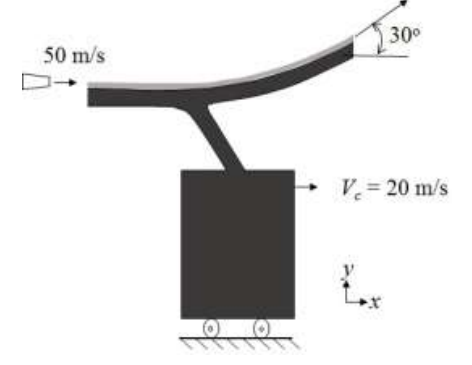
\includegraphics[width=0.5\linewidth]{figs/Q9.png}
\end{figure}\\
\item Capillary waves are generated in the sea. The speed of propagation \brak{C} of these waves is known to be a function of density $\brak{\rho}$, wave length $\brak{\lambda}$, and surface tension $\brak{\sigma}$. Assume, $\rho$ and $\lambda$ to be constant. If the surface tension is doubled, in the functional form of the relevant non-dimensional group, the percentage increase in propagation speed \brak{C} is $\_\_\_\_$. \\
\item Consider a fully developed, two-dimensional and steady flow of a viscous fluid between two fixed parallel plates separated by a distance of 30 mm. The dynamic viscosity of the fluid is 0.01 kg/m-s and the pressure drop per unit length is 300 Pa/m. The fluid velocity at a distance of 10 mm from the bottom plate, in m/s, is $\_\_\_\_$. \\
\item A 2.6 gram smooth table-tennis (ping-pong) ball has a diameter of 38 mm. Density $\brak{\rho}$ of air is 1.2 kg/$\text{m}^3$. Neglect the effect of gravity. Take coefficient of drag as 0.5. If the ball is struck with an initial velocity of 30 m/s, the initial deceleration, in m/$\text{s}^2$, is $\_\_\_\_$. \\
\item On a flat plate, transition from laminar to turbulent boundary layer occurred at a critical Reynolds number \brak{\text{Re}_{\text{cr}}}. The empirical relations for the laminar and turbulent boundary layer thickness are given by $\frac{\delta_{lam}}{x} = 5.48 \text{Re}_{x}^{-0.5}$ and $\frac{\delta_{turb}}{x} = 0.37 \text{Re}_{x}^{-0.2}$, respectively. The ratio of laminar to turbulent boundary layer thickness, at the location of transition, is 0.3.
The value of $\text{Re}_{\text{cr}}$ is $\_\_\_\_$. \\
			 \end{enumerate}
			 \end{document}
  
